\documentclass[a4paper,11pt]{article}

\usepackage[utf8]{inputenc}
\usepackage[T1]{fontenc}
\usepackage[french]{babel}
\usepackage{lmodern}
\usepackage{microtype}
\usepackage{graphicx}
\usepackage{hyperref}
\usepackage{xcolor}
\usepackage{tcolorbox}
\usepackage{enumitem}
\usepackage{geometry}
\usepackage{fancyhdr}
\usepackage[table]{xcolor}
\usepackage{booktabs}
\usepackage{array}
\usepackage{tabularx}
\usepackage{listings}
\usepackage{fancyvrb}
\usepackage{multicol}

\geometry{margin=2cm, top=2.5cm, bottom=2.5cm}
\setlength{\headheight}{14pt}

\definecolor{titlecolor}{RGB}{0, 90, 160}
\definecolor{sectitlecolor}{RGB}{5, 100, 175}
\definecolor{subsectitlecolor}{RGB}{10, 110, 190}
\definecolor{definitionbg}{RGB}{240, 248, 255}
\definecolor{examplebg}{RGB}{245, 255, 245}
\definecolor{warningbg}{RGB}{255, 245, 245}
\definecolor{benefitbg}{RGB}{255, 253, 235}
\definecolor{codecolor}{RGB}{240, 240, 240}
\definecolor{codekeyword}{RGB}{0, 0, 128}
\definecolor{codestring}{RGB}{163, 21, 21}
\definecolor{codecomment}{RGB}{0, 128, 0}
\definecolor{todobg}{RGB}{255, 235, 235}
\definecolor{collabg}{RGB}{245, 240, 255}

\lstset{
  basicstyle=\ttfamily\footnotesize,
  backgroundcolor=\color{codecolor},
  keywordstyle=\color{codekeyword}\bfseries,
  stringstyle=\color{codestring},
  commentstyle=\color{codecomment}\itshape,
  breaklines=true,
  showstringspaces=false,
  frame=single,
  tabsize=2,
  captionpos=b
}

\pagestyle{fancy}
\fancyhf{}
\fancyhead[L]{\textit{Lab 3 --- Le monolithe modulaire}}
\fancyhead[R]{\textit{Architectures Logicielles}}
\fancyfoot[C]{\thepage}
\fancyfoot[L]{\textit{Dr. El Hadji Bassirou TOURE}}
\fancyfoot[R]{\textit{DMI/FST/UCAD}}
\renewcommand{\headrulewidth}{0.4pt}
\renewcommand{\footrulewidth}{0.4pt}

\newtcolorbox{concept}{
  colback=definitionbg, colframe=sectitlecolor,
  title=Concept fondamental, fonttitle=\bfseries
}
\newtcolorbox{intuition}{
  colback=examplebg, colframe=green!75!black,
  title=Intuition, fonttitle=\bfseries
}
\newtcolorbox{exemple}{
  colback=orange!5!white, colframe=orange!75!black,
  title=Exemple, fonttitle=\bfseries, fontupper=\footnotesize
}
\newtcolorbox{pointcle}{
  colback=benefitbg, colframe=orange!70!black,
  title=Point cle a retenir, fonttitle=\bfseries
}
\newtcolorbox{warningbox}{
  colback=warningbg, colframe=red!70!black,
  title=Point d'attention, fonttitle=\bfseries
}
\newtcolorbox{benefitbox}{
  colback=benefitbg, colframe=green!70!black,
  title=Benefice, fonttitle=\bfseries
}
\newtcolorbox{todobox}{
  colback=todobg, colframe=red!60!black,
  title=Tache a realiser, fonttitle=\bfseries\scriptsize, fontupper=\small
}
\newtcolorbox{collabox}{
  colback=collabg, colframe=violet!70!black,
  title=Qui pilote cette section ?, fonttitle=\bfseries\scriptsize, fontupper=\small
}
\newtcolorbox{tagbox}{
  colback=yellow!15, colframe=yellow!50!black,
  title=Jalon Git, fonttitle=\bfseries\scriptsize, fontupper=\small
}

\lstset{
  basicstyle=\tiny\ttfamily,
  keywordstyle=\tiny\ttfamily\bfseries\color{codekeyword},
  commentstyle=\tiny\ttfamily\itshape\color{codecomment},
  stringstyle=\tiny\ttfamily\color{codestring}
}

\usepackage[explicit]{titlesec}
\titleformat{\section}
  {\Large\bfseries\color{titlecolor}}{\thesection}{0.5em}{#1}
\titleformat{\subsection}
  {\large\bfseries\color{sectitlecolor}}{\thesubsection}{0.5em}{#1}
\titleformat{\subsubsection}
  {\normalsize\bfseries\color{subsectitlecolor}}{\thesubsubsection}{0.5em}{#1}

\title{\textcolor{titlecolor}{\Huge\textbf{Lab 3 --- Le monolithe modulaire}}\\[0.5em]
       \textcolor{sectitlecolor}{\LARGE Des frontières entre les métiers, gardées par un test}}
\author{Dr. El Hadji Bassirou TOURE\\
        Département de Mathématiques et Informatique\\
        Faculté des Sciences et Techniques\\
        Université Cheikh Anta Diop}
\date{Année universitaire 2026--2027}

\begin{document}

\maketitle
\thispagestyle{empty}

\begin{abstract}
\noindent L'hexagone du Lab 2 protège votre métier de la technique --- mais
tous les métiers de SénResto cohabitent dans le même hexagone, libres de
s'appeler et de se mélanger. Ce lab trace les frontières manquantes : le
domaine est découpé en \textbf{cinq modules} (catalogue, commandes,
livraison, paiement, notifications) suivant ses \emph{bounded contexts},
chaque membre du groupe devenant \textbf{propriétaire d'un module}.
\textbf{Spring Modulith} transforme ces frontières en propriété vérifiée :
un test, \texttt{verify()}, casse le build à la moindre violation. Les
modules collaborent de deux façons que vous apprendrez à choisir : l'appel
direct d'API publique quand il faut une réponse, et les \textbf{événements
internes} quand on informe --- le module \texttt{paiement} naîtra d'ailleurs
en s'abonnant à un événement, sans modifier une ligne du module qui le
publie. Comme toujours : les 8 tests existants restent verts, et le
frontend ne remarque rien.
\end{abstract}

\begin{benefitbox}
À l'issue de ce lab, vous saurez :
\begin{itemize}[nosep]
  \item découper un domaine en \textbf{bounded contexts} en écoutant où le
        vocabulaire change de sens ;
  \item structurer un module Spring Modulith : API publique au paquetage
        racine, implémentation dans \texttt{interne/} ;
  \item faire garder les frontières \textbf{par le build}
        (\texttt{ApplicationModules.verify()}) --- et lire ses verdicts ;
  \item publier et écouter des \textbf{événements métier internes}, et
        choisir entre événement et appel direct.
\end{itemize}
\end{benefitbox}

\begin{warningbox}
\textbf{Prérequis avant la séance :}
\begin{itemize}[nosep]
  \item votre dépôt au tag \texttt{lab3-depart} (= \texttt{lab2-final},
        publié à l'ouverture) ;
  \item \texttt{./mvnw test} vert : \textbf{8 tests} (4 intégration +
        4 unitaires du domaine) ;
  \item connexion internet en début de séance (nouvelles dépendances
        Maven : Spring Modulith).
\end{itemize}
\end{warningbox}

\tableofcontents
\newpage

% =====================================================================
\section{Le constat : cartographier les mélanges}
% =====================================================================

\begin{intuition}
Une grande maison sans murs intérieurs fonctionne très bien... pour une
personne. À cinq, chacun a besoin de sa chambre. Votre domaine est cette
maison : avant de monter les murs, dessinons le plan --- qui vit où, et
qui traverse actuellement le salon de qui.
\end{intuition}

\subsection{Exercice (15 minutes, en groupe)}

Parcourez \texttt{domaine/} et remplissez ce tableau : pour chaque classe,
son futur module, et les autres classes qu'elle touche directement.

\begin{center}
\small
\begin{tabular}{p{0.30\textwidth}p{0.22\textwidth}p{0.34\textwidth}}
\toprule
\textbf{Classe actuelle} & \textbf{Futur module} & \textbf{Elle touche à...} \\
\midrule
\texttt{CommandeMetier} & commandes & \\
\texttt{RestaurantMetier} & catalogue & \\
\texttt{LivreurMetier} & livraison & \\
\texttt{CalculateurEta} & livraison & \\
\texttt{QuartiersDakar} & ? (discutez !) & \\
\texttt{NotificationsPort} & notifications & \\
\bottomrule
\end{tabular}
\end{center}

Deux découvertes attendues. D'abord, \texttt{CommandeMetier} touche à
\emph{tout} : plats du catalogue, livreurs, notifications --- c'est le
carrefour, et c'est normal : commander \emph{orchestre}. Ensuite, le cas
\texttt{QuartiersDakar} n'a pas de réponse évidente : les frais concernent
les commandes, les GPS concernent la livraison. C'est votre première vraie
décision de frontière --- matière à ADR (notre choix de référence : le
module \texttt{livraison} possède les quartiers et expose ce dont
\texttt{commandes} a besoin via son API publique ; d'autres choix se
défendent).

% =====================================================================
\section{Les concepts : modules et gardien}
% =====================================================================

\begin{concept}
\textbf{Bounded context.} Une zone du domaine où les mots ont \emph{un}
sens précis et le modèle est cohérent. La frontière passe où \textbf{le
vocabulaire change de sens} : « commande » ne désigne pas la même chose
pour Commandes (panier, statut), Livraison (course, ETA) et Paiement
(montant à encaisser). Cinq contextes chez SénResto : catalogue, commandes,
livraison, paiement, notifications --- un par membre.
\end{concept}

\begin{concept}
\textbf{Module Spring Modulith.} Chaque paquetage directement sous
l'application est un \emph{module}. Son paquetage racine est son
\textbf{API publique} (types accessibles aux autres modules, événements
compris) ; tout sous-paquetage --- par convention \texttt{interne/} ---
est \textbf{invisible} des autres modules. Et cette règle n'est pas un
v\oe u pieux : le test \texttt{ApplicationModules.verify()} casse le
build à la moindre violation, fichier et ligne à l'appui.
\end{concept}

\begin{figure}[h]
\centering
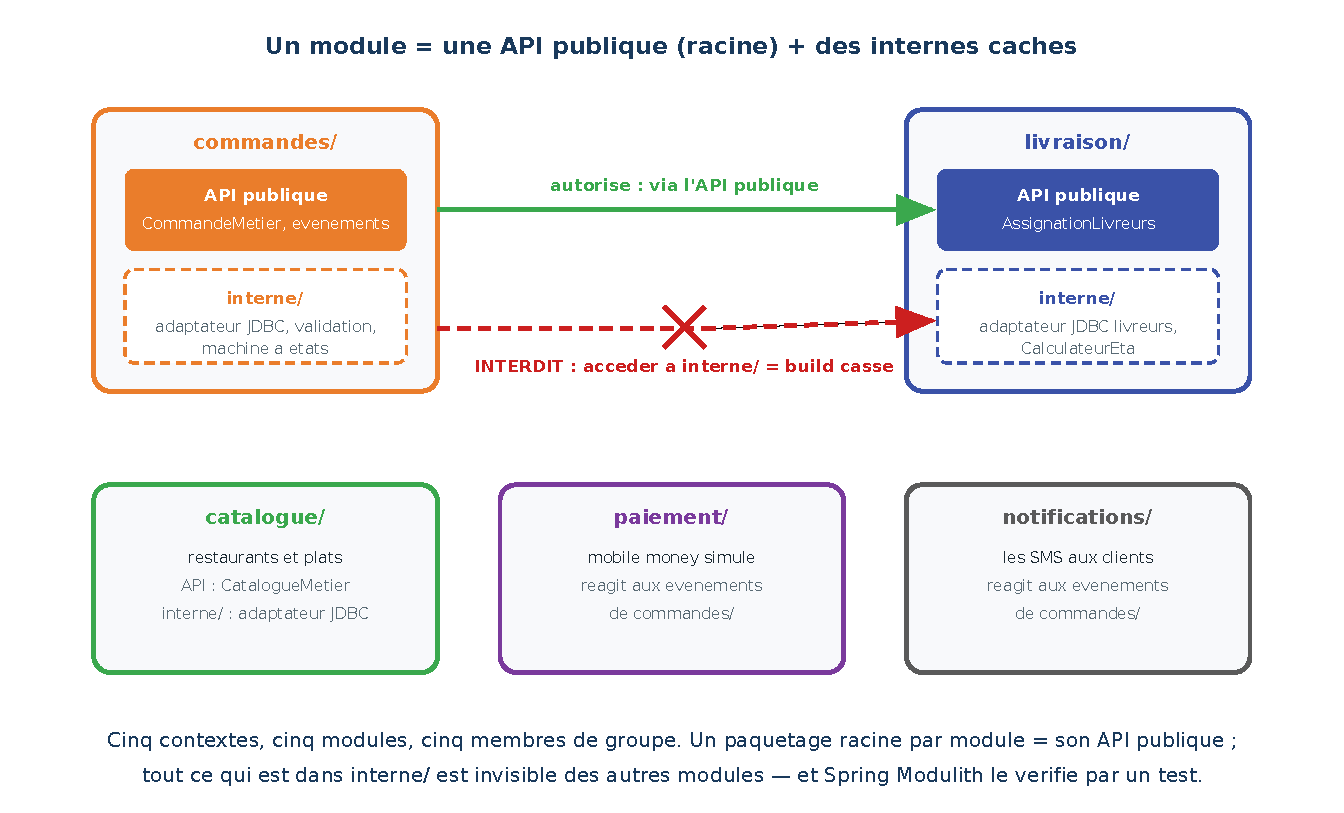
\includegraphics[width=0.85\textwidth]{figs/figG_modules.pdf}
\caption{La cible : cinq modules, API publiques et internes cachés.}
\end{figure}

\begin{concept}
\textbf{Le noyau partagé (shared kernel).} Certains types servent
plusieurs modules --- ici, les exceptions métier que \texttt{rest}
traduit en HTTP et que \texttt{catalogue} comme \texttt{commandes}
lèvent. Les loger dans \texttt{commandes} créerait
\texttt{catalogue} $\to$ \texttt{commandes} $\to$ \texttt{catalogue} :
un \textbf{cycle}, que \texttt{verify()} refuse. Le remède DDD : un
petit module \texttt{partage}, dont tout le monde peut dépendre et qui
ne dépend de personne. Anecdote véridique : ce cycle a été
\emph{réellement détecté par \texttt{verify()}} pendant la conception de
ce corrigé --- le gardien ne fait pas de politesse, même à l'enseignant.
\end{concept}

\subsection{La cible : la nouvelle carte des paquetages}

\begin{lstlisting}[language=bash]
sn/ucad/senresto/
|-- SenRestoApplication.java
|-- catalogue/
|   |-- CatalogueMetier.java              <- API publique
|   \-- interne/
|       |-- StockageCatalogue.java  (interface, pour les tests in-memory)
|       |-- AdaptateurCatalogueJdbc.java
|       \-- ConfigurationCatalogue.java
|-- commandes/
|   |-- CommandeMetier.java               <- API publique
|   |-- CommandeRequete.java  ChangementStatutRequete.java
|   |-- CommandeCreee.java  CommandeConfirmee.java  CommandeStatutChangee.java
|   |-- PublicationEvenements.java
|   \-- interne/
|       |-- StockageCommandes.java
|       |-- AdaptateurCommandesJdbc.java
|       |-- PublicationEvenementsSpring.java
|       \-- ConfigurationCommandes.java
|-- livraison/
|   |-- AssignationLivreurs.java  Assignation.java   <- API publique
|   |-- QuartiersDakar.java
|   \-- interne/
|       |-- StockageLivreurs.java
|       |-- AdaptateurLivreursJdbc.java
|       |-- CalculateurEta.java
|       \-- ConfigurationLivraison.java
|-- paiement/
|   \-- interne/
|       \-- EcouteurPaiement.java         <- nait d'un evenement
|-- partage/                              <- le noyau partage (shared kernel)
|   |-- ValidationException.java  IntrouvableException.java
|   \-- ConflitException.java
|-- notifications/
|   \-- interne/
|       |-- EcouteurNotifications.java
|       \-- AdaptateurSmsConsole.java
\-- rest/
    |-- SenRestoController.java  GestionnaireErreurs.java
\end{lstlisting}

\begin{warningbox}
Le lab conserve l'esprit hexagonal \emph{à l'intérieur} de chaque module
(le métier au centre, les adaptateurs en \texttt{interne/}) mais simplifie
le cérémonial : les ports explicites du Lab 2 ne sont conservés que là où
ils servent encore (tests in-memory de \texttt{commandes}). C'est un choix
d'équilibre assumé --- discutez-le, c'est une excellente ligne d'ADR.
\end{warningbox}

% =====================================================================
\section{Etape 1 --- Monter les murs}
% =====================================================================

\begin{collabox}
Chaque membre devient \textbf{propriétaire d'un module} : le Doyen ---
\texttt{commandes} ; l'Huissier --- \texttt{livraison} ; le Rédacteur ---
\texttt{catalogue} ; le Notaire --- \texttt{notifications} ;
l'Appariteur --- \texttt{paiement} (qui attendra l'étape 2 : son module
naît des événements). À l'étape 1, chacun déménage ses classes chez lui.
\end{collabox}

\subsection{Les dépendances Modulith}

Dans le \texttt{pom.xml}, ajoutez le BOM et les deux artefacts :

\begin{lstlisting}[language=xml]
<dependencyManagement>
  <dependencies>
    <dependency>
      <groupId>org.springframework.modulith</groupId>
      <artifactId>spring-modulith-bom</artifactId>
      <version>1.2.5</version>
      <type>pom</type>
      <scope>import</scope>
    </dependency>
  </dependencies>
</dependencyManagement>
\end{lstlisting}

\begin{lstlisting}[language=xml]
<dependency>
  <groupId>org.springframework.modulith</groupId>
  <artifactId>spring-modulith-starter-core</artifactId>
</dependency>
<dependency>
  <groupId>org.springframework.modulith</groupId>
  <artifactId>spring-modulith-starter-test</artifactId>
  <scope>test</scope>
</dependency>
\end{lstlisting}

\subsection{Le neuvième juge}

Avant même de déménager, installez le gardien --- il sera rouge, c'est
normal, et vous le regarderez passer au vert module par module :

\begin{lstlisting}[language=java]
package sn.ucad.senresto;

import org.junit.jupiter.api.Test;
import org.springframework.modulith.core.ApplicationModules;

class ModulithArchitectureTest {

    @Test
    void lesFrontieresDesModulesSontRespectees() {
        ApplicationModules modules = ApplicationModules.of(SenRestoApplication.class);
        modules.forEach(System.out::println);   // la carte, lue depuis le code
        modules.verify();                       // le verdict
    }
}
\end{lstlisting}

\subsection{Le déménagement}

Chaque propriétaire crée son paquetage et son \texttt{interne/}, y déplace
ses classes (l'IDE fait les imports), en appliquant la règle : \emph{ce que
les autres modules utilisent} reste à la racine, tout le reste descend dans
\texttt{interne/}. Cas guidés :

\begin{itemize}[nosep]
  \item \textbf{livraison} expose \texttt{AssignationLivreurs} et le
        record \texttt{Assignation}. Attention à la conception de
        l'API : pas de méthodes \texttt{premierDisponible} puis
        \texttt{reserver} séparées, mais une seule opération
        \texttt{assigner(quartier)} qui choisit,
        calcule l'ETA et réserve. Pourquoi ? Parce que
        \texttt{CalculateurEta} descend en \texttt{interne/} : si
        \texttt{commandes} devait calculer l'ETA lui-même, il lui faudrait
        ce secret --- violation immédiate. \emph{L'ETA est un secret de
        livraison} : c'est l'encapsulation qui dessine l'API ;
  \item \textbf{commandes} garde à sa racine \texttt{CommandeMetier}, les
        deux requêtes et les trois exceptions (le module \texttt{rest} les
        traduit en HTTP) ;
  \item \textbf{catalogue} expose \texttt{CatalogueMetier}
        (ex-\texttt{RestaurantMetier}, renommé au passage : le vocabulaire
        du contexte) ;
  \item \texttt{CommandeMetier} appelle désormais
        \texttt{AssignationLivreurs} et \texttt{CatalogueMetier} --- des
        API publiques : autorisé, et \texttt{verify()} l'atteste ;
  \item la \texttt{ConfigurationDomaine} globale du Lab 2 disparaît :
        \textbf{chaque module assemble son propre métier} dans une
        \texttt{@Configuration} de son \texttt{interne/} --- les murs
        valent aussi pour l'assemblage.
\end{itemize}

\begin{warningbox}
\textbf{Le piège des classes fantômes.} Après un grand déménagement de
paquetages, lancez toujours \texttt{./mvnw clean test} --- pas
\texttt{test} seul. Maven compile les nouvelles sources mais ne supprime
jamais les \texttt{.class} des classes disparues : \texttt{verify()} et
Spring, qui lisent \texttt{target/classes}, verraient alors les
\emph{fantômes} de l'ancienne architecture (violations inexplicables,
doublons de beans). Vécu et diagnostiqué sur ce cours même.
\end{warningbox}

\begin{todobox}
\textbf{À réaliser --- étape 1} (une branche \texttt{feature/module-xxx}
par propriétaire) : les cinq paquetages montés (paiement encore vide, avec
un \texttt{package-info.java}), toutes les classes déménagées, le
\texttt{ModulithArchitectureTest} \textbf{vert}, les 8 tests existants
\textbf{verts}, le frontend intact.
\end{todobox}

\begin{tagbox}
9 tests verts (8 + verify) :
\begin{center}
\texttt{git tag lab3-etape1 \&\& git push origin lab3-etape1}
\end{center}
\end{tagbox}

% =====================================================================
\section{Etape 2 --- Les événements internes}
% =====================================================================

\begin{collabox}
\textbf{Le Doyen} fait publier \texttt{commandes}. \textbf{Le Notaire}
abonne \texttt{notifications}. \textbf{L'Appariteur} fait naître
\texttt{paiement}. \textbf{L'Huissier} et \textbf{le Rédacteur} vérifient
que leurs modules n'ont \emph{rien} à changer --- c'est aussi une leçon.
\end{collabox}

\begin{figure}[h]
\centering
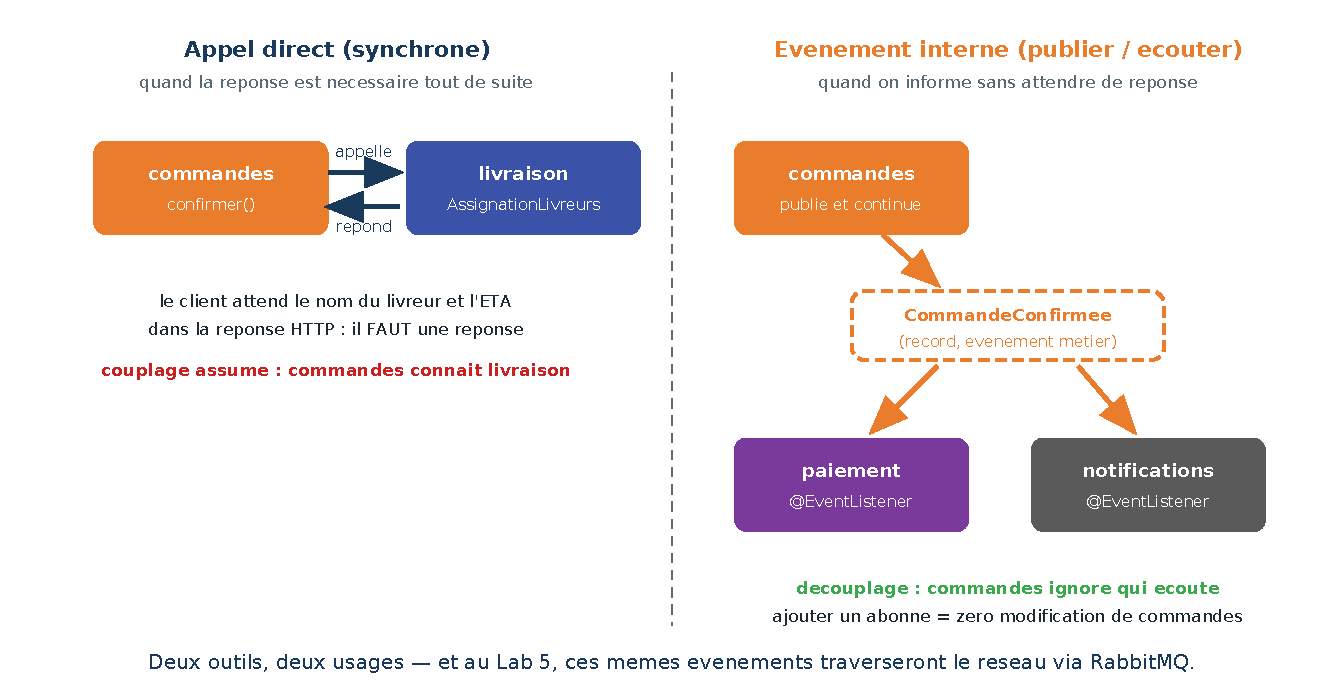
\includegraphics[width=0.78\textwidth]{figs/figH_appel_vs_evenement.pdf}
\caption{Appel direct quand il faut une réponse ; événement quand on informe.}
\end{figure}

\subsection{Commandes publie des faits}

Trois records dans la racine de \texttt{commandes} --- des faits passés,
nommés au participe :

\begin{lstlisting}[language=java]
public record CommandeCreee(long commandeId, String numero,
        String clientTelephone, String restaurantNom, int montantTotal) {}

public record CommandeConfirmee(long commandeId, String numero,
        String clientTelephone, int montantTotal,
        String livreurNom, int etaMinutes) {}

public record CommandeStatutChangee(long commandeId, String numero,
        String clientTelephone, String nouveauStatut) {}
\end{lstlisting}

Pour rester fidèle à l'hexagone, \texttt{CommandeMetier} ne dépend pas de
Spring : il publie via une petite interface de sa racine, dont
l'implémentation Spring vit en \texttt{interne/} :

\begin{lstlisting}[language=java]
// commandes/PublicationEvenements.java  (racine)
public interface PublicationEvenements {
    void publier(Object evenement);
}

// commandes/interne/PublicationEvenementsSpring.java
@Component
class PublicationEvenementsSpring implements PublicationEvenements {
    private final ApplicationEventPublisher spring;
    PublicationEvenementsSpring(ApplicationEventPublisher spring) { this.spring = spring; }
    @Override public void publier(Object evenement) { spring.publishEvent(evenement); }
}
\end{lstlisting}

Dans \texttt{CommandeMetier}, les appels directs aux notifications sont
remplacés par des publications --- et la dépendance aux notifications
\textbf{disparaît} de son constructeur :

\begin{lstlisting}[language=java]
// creer() : a la place de notifications.envoyerSms(...)
evenements.publier(new CommandeCreee(id, numero, clientTelephone,
        (String) plat.get("restaurant_nom"), montantTotal));
\end{lstlisting}

\subsection{Notifications s'abonne --- memes SMS qu'avant}

\begin{lstlisting}[language=java]
// notifications/interne/EcouteurNotifications.java
@Component
class EcouteurNotifications {

    private final AdaptateurSmsConsole sms;

    EcouteurNotifications(AdaptateurSmsConsole sms) { this.sms = sms; }

    @EventListener
    void quandCommandeCreee(CommandeCreee evt) {
        sms.envoyerSms(evt.clientTelephone(), "Commande " + evt.numero()
                + " recue chez " + evt.restaurantNom()
                + " -- total " + evt.montantTotal() + " FCFA");
    }
    // quandCommandeConfirmee(...), quandStatutChange(...) : meme principe,
    // MEMES textes de SMS qu'au depart -- le comportement observable
    // ne change pas (les evenements Spring sont synchrones par defaut).
}
\end{lstlisting}

\subsection{Paiement nait d'un evenement}

Le moment pédagogique du lab : l'Appariteur crée le module
\texttt{paiement} \textbf{sans qu'aucun autre module ne soit modifié} ---
la preuve vivante du découplage :

\begin{lstlisting}[language=java]
// paiement/interne/EcouteurPaiement.java
@Component
class EcouteurPaiement {

    @EventListener
    void quandCommandeConfirmee(CommandeConfirmee evt) {
        System.out.println("[PAIEMENT] Encaissement mobile money simule : "
                + evt.montantTotal() + " FCFA pour la commande " + evt.numero());
    }
}
\end{lstlisting}

\begin{exemple}
Passez une commande depuis le frontend et confirmez-la : dans la console,
le \texttt{[SMS]} habituel est maintenant suivi d'une ligne
\texttt{[PAIEMENT]}. Deux modules ont réagi au même fait --- et
\texttt{commandes} l'ignore superbement. Au Lab 5, Wave et Orange Money
« réels » (simulés) remplaceront ce \texttt{System.out}, avec webhooks et
idempotence.
\end{exemple}

\begin{warningbox}
Les tests unitaires de \texttt{CommandeMetier} évoluent : le port
notifications disparaît de son constructeur au profit de
\texttt{PublicationEvenements}. En test, un enregistreur suffit ---
\texttt{evenements.add(evt)} dans une liste --- et les assertions
deviennent plus expressives encore : \emph{vérifier qu'un fait a été
publié} plutôt qu'un SMS envoyé.
\end{warningbox}

\begin{todobox}
\textbf{À réaliser --- étape 2 :}
\begin{itemize}[nosep]
  \item Le Doyen : les 3 records, \texttt{PublicationEvenements} + son
        adaptateur Spring, \texttt{CommandeMetier} qui publie ;
  \item Le Notaire : \texttt{EcouteurNotifications}, 3 écouteurs,
        \textbf{mêmes textes de SMS} (les tests d'intégration y veillent) ;
  \item L'Appariteur : le module \texttt{paiement} complet ;
  \item L'Huissier et le Rédacteur : adaptation des tests unitaires de
        \texttt{commandes} (enregistreur d'événements), et vérification
        que \texttt{livraison} et \texttt{catalogue} n'ont pas bougé ;
  \item Tous : \texttt{./mvnw test} --- 9 juges verts.
\end{itemize}
\end{todobox}

\begin{tagbox}
\begin{center}
\texttt{git tag lab3-etape2 \&\& git push origin lab3-etape2}
\end{center}
\end{tagbox}

% =====================================================================
\section{Etape finale --- Eprouver le gardien}
% =====================================================================

\begin{collabox}
\textbf{Tous ensemble}, au vidéoprojecteur du groupe : cette étape est une
expérience, pas une production.
\end{collabox}

\subsection{La violation volontaire}

Dans \texttt{CommandeMetier}, ajoutez volontairement un import interdit :

\begin{lstlisting}[language=java]
import sn.ucad.senresto.livraison.interne.CalculateurEta;   // INTERDIT !
\end{lstlisting}

Utilisez-le n'importe où, lancez \texttt{./mvnw test}, et \textbf{lisez le
verdict} de \texttt{verify()} : le module fautif, le type visé, la
violation nommée. Puis retirez l'import. Vous venez de voir la différence
entre une convention (qui s'érode) et une architecture (qui casse le
build). Recommencez si un membre du groupe est sceptique --- c'est fait
pour ça.

\subsection{La documentation qui ne ment pas}

Ajoutez au \texttt{ModulithArchitectureTest} :

\begin{lstlisting}[language=java]
@Test
void genererLaDocumentationDesModules() {
    new Documenter(ApplicationModules.of(SenRestoApplication.class))
            .writeModulesAsPlantUml()
            .writeIndividualModulesAsPlantUml();
}
\end{lstlisting}

Les diagrammes apparaissent dans \texttt{target/spring-modulith-docs/} :
une carte des modules \textbf{générée depuis le code}, donc toujours
vraie. Le Rédacteur la joint au dépôt (\texttt{docs/modules/}) --- c'est
la pièce jointe rêvée de l'ADR.

\begin{todobox}
\textbf{À réaliser --- étape finale :} l'expérience de violation faite et
défaite (elle doit apparaître dans l'historique Git : le commit qui casse,
le commit qui répare --- c'est votre preuve de manipulation) ; la
documentation générée et versionnée ; les 9 juges verts ; le parcours
frontend complet avec la ligne \texttt{[PAIEMENT]} dans la console.
\end{todobox}

\begin{tagbox}
\begin{center}
\texttt{git tag lab3-final \&\& git push origin lab3-final}
\end{center}
\end{tagbox}

% =====================================================================
\section{Recapitulatif : qui a fait quoi}
% =====================================================================

\begin{center}
\small
\begin{tabular}{p{0.16\textwidth}p{0.26\textwidth}p{0.28\textwidth}p{0.20\textwidth}}
\toprule
\textbf{Rôle} & \textbf{Étape 1} & \textbf{Étape 2} & \textbf{Étape finale} \\
\midrule
Le Doyen & module \texttt{commandes} & records + publications & tag final, ADR \\
\addlinespace
L'Huissier & module \texttt{livraison}, API \texttt{AssignationLivreurs} & vérif. « rien à changer » + tests unitaires & violation volontaire \\
\addlinespace
Le Rédacteur & module \texttt{catalogue} & vérif. + tests unitaires & documentation générée \\
\addlinespace
Le Notaire & module \texttt{notifications} & les 3 écouteurs & relecture des SMS \\
\addlinespace
L'Appariteur & \texttt{paiement} (coquille) & le module \texttt{paiement} né d'un événement & démo \texttt{[PAIEMENT]} \\
\bottomrule
\end{tabular}
\end{center}

% =====================================================================
\section{L'ADR du jour}
% =====================================================================

L'\textbf{Architecte du jour} signe l'\textbf{ADR n\up{o}3 : « Comment
tracer les frontières des modules ? »}
(\texttt{docs/adr/adr-003-frontieres.md}). Matière obligatoire : la
décision \texttt{QuartiersDakar} (qui possède les quartiers, et pourquoi) ;
le choix appel direct pour \texttt{livraison} \emph{versus} événement pour
\texttt{paiement}/\texttt{notifications} (pourquoi pas tout en
événements ?). Alternatives sérieuses possibles : loger les exceptions dans chaque
module (duplication assumée) plutôt que dans \texttt{partage} ; tout-événements avec
enrichissement ; garder quatre modules sans \texttt{paiement}.
Conséquences négatives à assumer : la discipline des paquetages, les API
publiques à faire vivre, le risque de modules anémiques.

% =====================================================================
\section{Livrable et criteres de reussite}
% =====================================================================

\begin{center}
\small
\begin{tabular}{p{0.62\textwidth}p{0.28\textwidth}}
\toprule
\textbf{Critère} & \textbf{Vérification} \\
\midrule
Les 4 tags du lab présents & \texttt{git tag} \\
9 juges verts sur \texttt{lab3-final} (8 tests + verify) & \texttt{./mvnw test} \\
Aucun import d'un \texttt{interne/} étranger & \texttt{verify()} + relecture \\
La violation volontaire dans l'historique (cassée puis réparée) & \texttt{git log} \\
Le module \texttt{paiement} né sans toucher \texttt{commandes} & \texttt{git diff} ciblé \\
Mêmes SMS qu'au départ, ligne \texttt{[PAIEMENT]} en plus & console \\
Documentation des modules versionnée & \texttt{docs/modules/} \\
ADR n\up{o}3 signé & \texttt{docs/adr/} \\
\bottomrule
\end{tabular}
\end{center}

% =====================================================================
\section{Vers le Lab 4 : le depart d'un module}
% =====================================================================

Votre monolithe est modulaire : frontières nettes, gardien vigilant,
collaboration par API et par événements. C'est exactement pour cette
raison que la suite devient \emph{possible} : la direction veut faire
évoluer le calcul d'itinéraires avec l'écosystème Python (géospatial,
data), et le déployer sans redéployer SénResto. Le module
\texttt{livraison} --- frontières déjà tracées, API déjà publique --- est
le candidat parfait à l'\textbf{extraction}. Au Lab 4 : le pattern
Strangler Fig, un microservice FastAPI, une carte Leaflet de Dakar...
et une panne instructive dont vous vous souviendrez. Votre
\texttt{lab3-final} en sera le point de départ.

\vspace{1em}
\begin{center}
\textit{Fin du Lab 3 --- Dr. El Hadji Bassirou TOURE --- DMI/FST/UCAD}
\end{center}

\end{document}
